\begin{frame}
\frametitle{Problem Statement-Miscellenous}
\begin{enumerate}[label=(\roman*)]
\item In a circular table cover of radius 32 cm, a design is formed leaving an equilateral $\triangle{ABC}$
in the middle. Find the area of the design.\\
\end{enumerate}
\textbf{Soln:}\\
  Given: R=32cm\\
\url{https://github.com/Rajolep/_Geometry/blob/master/codes/miscel.py}
\begin{figure}
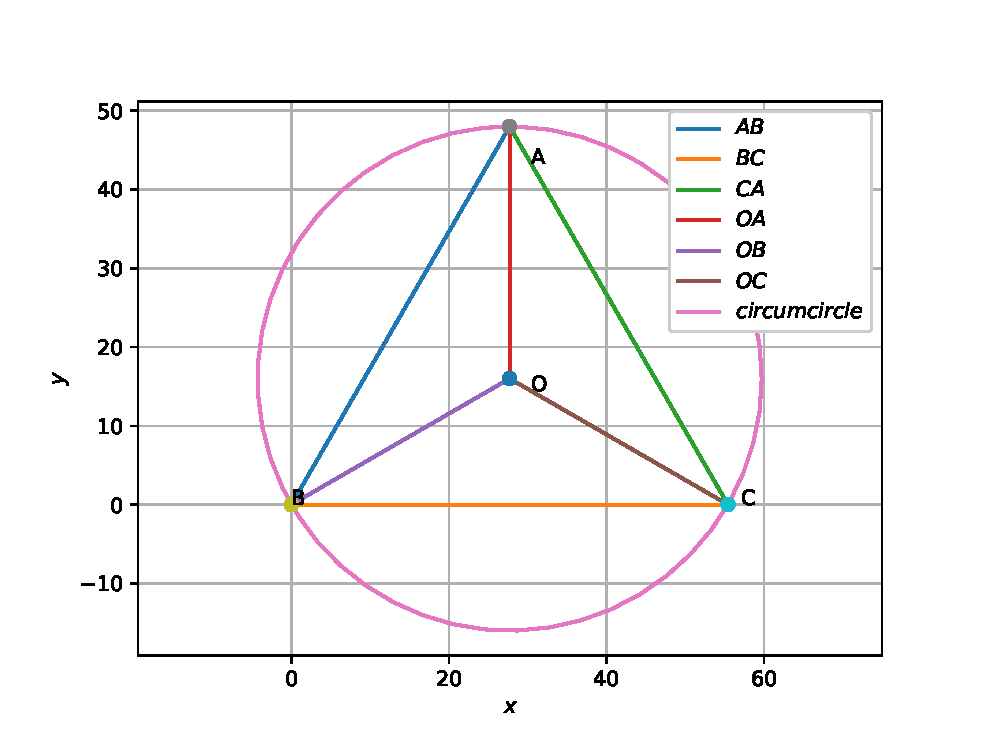
\includegraphics[scale=0.3]{./figs/misc.eps}
\end{figure}
\end{frame}
\begin{frame}
\url{https://github.com/Rajolep/_Geometry/blob/master/figs/miscell.tex}
\begin{figure}
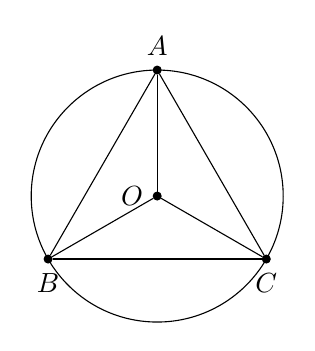
\begin{tikzpicture}
[scale =0.05,>=stealth,point/.style = {draw, circle, fill = black, inner sep = 1pt},]
\def\rad{32}
\coordinate [point, label={left: $O$ }] (O) at (27.712,16);
\draw (O) circle (\rad);
\node (B) at (0,0)[point,label=below :$B$] {};
\node (C) at (55.42,0)[point,label=below :$C$] {};
\node (A) at (27.712,48)[point,label=above :$A$] {};
\draw (A)--(C);
\draw (O)--(C);
\draw (O)--(B);
\draw (A)--(O);
\draw (A)--(B);
\draw (B)--(C);

\end{tikzpicture}

\end{figure}
%\begin{align*}
%\triangle{BOC} = 120\degree \\
%BO=OC=32\\
%BC=\sqrt{(BO)^2+(OC)^2-2(BO)(OC)\cos(120)}=55.425\\
%a=\sqrt{(2R)^2-2(R)^2)\cos{120}}\\
%s=\frac{a+b+c}{2}\\
%\end{{align*}
%Area of design = $\pi(R)(R)$ - $\sqrt{s(s-a)(s-b)(s-c)}$\\
%Area = 1886.81
\end{frame}